\chapter{流形之间的关系}
\label{chap:manifold-relations}

球面与椭球面看起来不同，一个圆，一个扁；可是把椭球面沿三个坐标轴分别缩放，就能毫无撕裂、毫无折叠地变成球面，反过来也一样。另一方面，圆周放在平面里是一条光滑的闭曲线，而一条在原点自交的“8”字形曲线，虽然也是由光滑参数化画出来的，却在交叉点处不像一段曲线。前一个例子问的是两个流形是否“本质上相同”，后一个问的是一个对象能否作为另一个流形中的光滑子流形。

上一章已经能计算映射的微分和秩。本章用这些工具研究流形之间的两种关系。第~\ref{sec:mrel-diffeomorphisms}节用微分同胚表达两个流形具有相同的光滑结构，并说明微分可逆只给出局部的可逆性。第~\ref{sec:mrel-local-structure}节考察映射在一点附近的结构：微分处处单射的浸入保留方向，处处满射的淹没覆盖方向；在秩保持不变的邻域中，常秩定理把映射化为最简单的坐标形式。

局部结构还不足以描述包含关系，“8”字形曲线就是局部处处保留方向、整体却不像子空间的例子。第~\ref{sec:mrel-embedded-submanifolds}节因此在浸入之上加入到像的同胚条件，得到嵌入，再用一部分坐标取零的局部模型刻画嵌入子流形，最后说明约束方程的微分满秩时，水平集自动成为这样的子流形；球面和正交矩阵组成的集合都由此得到。

本章只讨论无边界流形。带边界时，反函数定理在边界点处需要另外的处理，相应结论另核条件，只在必要处说明。微分同胚保持光滑结构，但不保持长度：区间$(0,1)$与整条实轴微分同胚，长度却一个有限、一个无限。比较长度和距离的等距关系，要在第~\ref{chap:riemannian-geometry}章引入黎曼度量之后讨论。

\section{微分同胚}
\label{sec:mrel-diffeomorphisms}

两个流形什么时候应当看作“同一个”光滑流形？集合论只问元素能否一一对应，拓扑只问邻近关系能否一一对应，而光滑流形还带有光滑结构，即哪些函数光滑、哪些曲线有速度。要说两个流形在光滑意义下相同，就要求有一个对应把这些信息双向保留下来。

\paragraph{定义}
保留光滑结构，意味着对应本身光滑，并且反过来的对应也光滑。

\begin{definition}[微分同胚]
\label{def:mrel-diffeomorphism}
设$M,N$是光滑流形。若$F:M\to N$是光滑双射，且逆映射$F^{-1}:N\to M$也光滑，则称$F$为\term{微分同胚}（diffeomorphism）。存在微分同胚时，称$M$与$N$微分同胚。
\end{definition}

微分同胚$F$把$N$上的光滑函数$g$对应到$M$上的光滑函数$g\circ F$，反过来$f\mapsto f\circ F^{-1}$，两种对应互逆。所以在两个流形上能谈论的“光滑对象”完全相同，只是名字换了。第~\ref{chap:manifold-maps}章又说明，光滑双射且逆光滑的映射把向量场一一推送为光滑向量场，所以微分同胚也保留了向量场。

\paragraph{三种对应的比较}
集合双射、同胚与微分同胚依次保留越来越多的信息，可以用例子看清每一层多出了什么。

只是集合双射，几乎什么都不保留。$\mathbb R$与$\mathbb R^2$的元素可以一一对应，但这样的双射不可能是同胚，因为维数是拓扑不变量；这一维数不变性需要较深的拓扑工具，这里不给出证明。同胚保留连通性、紧性这类拓扑性质，但不保留光滑性。$F(x)=x^3$是$\mathbb R$到自身的同胚，也是光滑双射，但逆映射$x^{1/3}$在原点不可微，所以$F$不是微分同胚。在$F$下，光滑函数$g(y)=y$对应到$g\circ F^{-1}$即$x^{1/3}$，不再光滑。

微分同胚是比较两个光滑结构的正确工具，而不是比较两个图册的写法。第~\ref{chap:manifold-basics}章指出，$\mathbb R$上的图$\chi(x)=x^3$与恒等图不光滑相容，记带$\chi$所决定结构的实轴为$\mathbb R_\chi$。恒等映射$\mathbb R\to\mathbb R_\chi$是同胚，但不是微分同胚。可是$G(x)=x^{1/3}$是从标准$\mathbb R$到$\mathbb R_\chi$的微分同胚：坐标表示是$\chi\circ G(x)=x$，逆映射的坐标表示是$G^{-1}\circ\chi^{-1}(z)=(z^{1/3})^3=z$，都光滑。所以这两个光滑结构不同，得到的光滑流形却微分同胚。

\paragraph{微分同胚的微分可逆}
微分同胚在每点的微分都是线性同构，这是链式法则的直接推论，也说明微分同胚的流形维数相同。

\begin{theorem}[微分同胚的微分]
\label{thm:mrel-diffeo-differential}
若$F:M\to N$是微分同胚，则对每个$p\in M$，$\mathrm dF_p:T_pM\to T_{F(p)}N$是线性同构，其逆为$\mathrm d(F^{-1})_{F(p)}$。特别地，$\dim M=\dim N$。
\end{theorem}

\begin{proof}
对$F^{-1}\circ F=\mathrm{id}_M$与$F\circ F^{-1}=\mathrm{id}_N$分别用链式法则，得$\mathrm d(F^{-1})_{F(p)}\circ\mathrm dF_p=\mathrm{id}_{T_pM}$与$\mathrm dF_p\circ\mathrm d(F^{-1})_{F(p)}=\mathrm{id}_{T_{F(p)}N}$。两个有限维空间之间存在互逆的线性映射，维数相同。
\end{proof}

\paragraph{反函数定理}
反过来，若只知道$\mathrm dF_p$可逆，能推出什么？在欧氏空间中，局部反函数定理说：Jacobian矩阵在一点可逆的连续可微映射，在该点附近有连续可微的逆。这一定理及隐函数定理可参考\BookChapterRef{chap:implicit-inverse-functions}{卷二第19章“隐函数与反函数”}；光滑映射的逆映射也光滑，因为逆映射的Jacobian矩阵$[\bm J_G]^{-1}$是光滑函数的复合，逐阶求导即可。借助坐标图，这一结论搬到流形上。

\begin{theorem}[流形上的反函数定理]
\label{thm:mrel-inverse-function}
设$M,N$是无边界光滑流形，$F:M\to N$光滑，$p\in M$，且$\mathrm dF_p$可逆。则存在$p$的开邻域$U$与$F(p)$的开邻域$V$，使$F|_U:U\to V$是微分同胚。
\end{theorem}

\begin{proof}
取包含$p$与$F(p)$的图，使$F(U_1)\subseteq V_1$。坐标表示$\hat F$在$\varphi(p)$处的Jacobian矩阵就是$\mathrm dF_p$的矩阵，可逆，于是两侧维数相同。由欧氏反函数定理，存在$\varphi(p)$的开邻域$\widehat U$与$\hat F(\varphi(p))$的开邻域$\widehat V$，使$\hat F:\widehat U\to\widehat V$是光滑双射且逆光滑。令$U=\varphi^{-1}(\widehat U)$，$V=\psi^{-1}(\widehat V)$，则$F|_U=\psi^{-1}\circ\hat F\circ\varphi$是三个微分同胚的复合。
\end{proof}

$\varphi(p)$在$\varphi(U_1)$的内部是这里不可缺少的。在半空间的边界点处，坐标表示的值域可能被迫落在半空间中，欧氏反函数定理给出的开邻域不再适用，所以本章把讨论限制在无边界情形。

\paragraph{局部可逆与整体双射}
若$F$在每点都满足定理~\ref{thm:mrel-inverse-function}的条件，就称它为\term{局部微分同胚}（local diffeomorphism）。局部微分同胚未必是微分同胚，因为反函数定理只给出局部的逆，不涉及整体是否一一对应。

映射$E:\mathbb R\to S^1$，$E(t)=(\cos t,\sin t)$，在角度图中坐标表示的导数为$1$，所以是局部微分同胚；但$E(t)=E(t+2\pi)$，它不是单射。圆周上的倍角映射$(\cos\theta,\sin\theta)\mapsto(\cos2\theta,\sin2\theta)$在角度坐标中是$\theta\mapsto2\theta$（相差$2\pi$的整数倍），导数为$2$，也是局部微分同胚，并且是满射，可每点恰有两个原像。这两个例子说明，导数处处可逆既不推出单射，也与满射无关。

缺的正是整体的一一对应。若局部微分同胚$F$还是双射，它就是微分同胚：逆映射$F^{-1}$在每点$q$附近与反函数定理给出的局部逆一致，局部逆光滑，所以$F^{-1}$光滑。类似地，单射的局部微分同胚是到其像的微分同胚，并且像是开集，因为每点的像都含有一个开邻域。

\paragraph{光滑结构相同不等于几何相同}
微分同胚只关心光滑结构，不关心长度与距离。映射$x\mapsto\tan(\pi(x-\tfrac12))$是$(0,1)$到$\mathbb R$的微分同胚，导数$\pi/\cos^2(\pi(x-\tfrac12))$处处为正，逆映射$y\mapsto\tfrac12+\tfrac1\pi\arctan y$也光滑。前者长度为$1$，后者无界。再如$x\mapsto2x$是$\mathbb R$到自身的微分同胚，把所有距离加倍。所以微分同胚的两个流形可以有完全不同的度量性质。保持长度的映射需要在切空间上先有内积，这样的等距映射在第~\ref{chap:riemannian-geometry}章讨论。

\section{映射的局部结构}
\label{sec:mrel-local-structure}

要判断一个映射的像或原像能否成为光滑子流形，先要看映射在一点附近怎样作用于方向。微分可能把非零的切向量送到零，丢失方向；可能达不到目标的全部方向；还可能在附近各点的秩不同。本节的$M,N$都是无边界光滑流形，维数分别为$m,n$，整体的拓扑条件留到下一节。

\subsection{浸入与淹没}
\label{sec:mrel-immersion-submersion}

\paragraph{定义}
线性代数里，矩阵的列线性无关时对应的映射是单射，行线性无关时是满射。下面两个矩阵分别属于这两类：
\[
\begin{bmatrix}1&0\\0&1\\1&1\end{bmatrix},\qquad
\begin{bmatrix}1&0&1\\0&1&1\end{bmatrix}.
\]
第一个是$3\times2$矩阵，秩为$2$，把$\mathbb R^2$单射地送进$\mathbb R^3$；第二个是$2\times3$矩阵，秩为$2$，把$\mathbb R^3$满射地压到$\mathbb R^2$上。对映射在每一点的微分提出这两种要求，就得到两类映射。

\begin{definition}[浸入与淹没]
\label{def:mrel-immersion-submersion}
设$F:M\to N$光滑。若对每个$p\in M$，$\mathrm dF_p$都是单射，则称$F$为\term{浸入}（immersion）；若对每个$p\in M$，$\mathrm dF_p$都是满射，则称$F$为\term{淹没}（submersion）。
\end{definition}

浸入不丢失方向：经过$p$的两个不同速度被送到$F(p)$处的两个不同速度。淹没覆盖方向：$F(p)$处的任何速度都是某个$p$处速度的像。用秩表达，浸入在每点秩为$m$，淹没在每点秩为$n$。

单射要求$m\leq n$，满射要求$m\geq n$，所以浸入只能从低维到高维或同维，淹没只能从高维到低维或同维。同维时两者一致，由反函数定理都等价于局部微分同胚。

\paragraph{例子}
曲线$\gamma:I\to M$是浸入，当且仅当速度处处非零。图~\ref{fig:mrel-cusp-velocity}比较了两条平面曲线。$E(t)=(\cos t,\sin t)$作为$\mathbb R\to\mathbb R^2$的映射，速度$(-\sin t,\cos t)$的长度恒为$1$，处处非零，是浸入。

$\beta(t)=(t^2,t^3)$的速度是$(2t,3t^2)$，在$t=0$处为零，不是浸入。它的像是曲线$y_2^2=y_1^3$，在原点有一个尖点。接近原点时速度越来越小，曲线的方向在原点处从一支突然转到另一支，这正是速度为零允许发生的事。

\begin{BookInlineFigure}
  \centering
  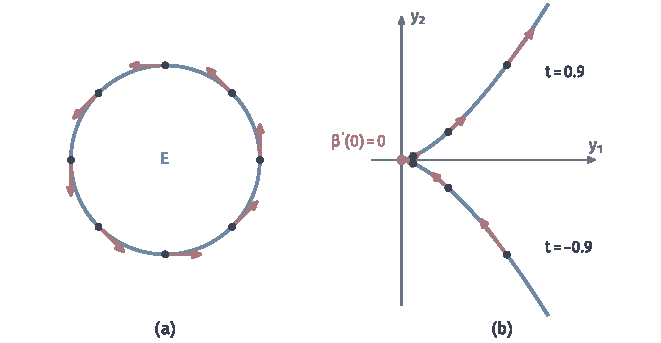
\includegraphics[width=112mm]{figures/04-spaces-measures-and-geometry/04-manifolds/matplotlib/mrel-cusp-velocity/figure.pdf}
  \caption{速度是否为零。(a)$E(t)=(\cos t,\sin t)$的速度（红箭头）长度恒为$1$，$E$是浸入。(b)$\beta(t)=(t^2,t^3)$在$t=\pm0.3,\pm0.6,\pm0.9$处的速度按真实长度的$0.12$倍画出，越接近原点越短；原点处速度为零，曲线出现尖点。}
  \label{fig:mrel-cusp-velocity}
\end{BookInlineFigure}

高维的浸入也可以手算。北极球极投影的逆把坐标$\bm u=(u_1,u_2)$送到$\mathbb R^3$，记$\rho=u_1^2+u_2^2$，
\[
\sigma_N^{-1}(\bm u)=\frac{(2u_1,\ 2u_2,\ \rho-1)}{\rho+1}.
\]
在$\bm u=(0,3)$处，第一列已在第~\ref{chap:manifold-basics}章算出是$(\tfrac15,0,0)$。第二列对$u_2$求导，三个分量分别是
\[
\frac{-4u_1u_2}{(\rho+1)^2}=0,\qquad
\frac{2(\rho+1)-4u_2^2}{(\rho+1)^2}=-\frac4{25},\qquad
\frac{4u_2}{(\rho+1)^2}=\frac3{25}.
\]

于是在这一点的Jacobian矩阵及其秩是
\[
\bm J=\begin{bmatrix}1/5&0\\0&-4/25\\0&3/25\end{bmatrix},\qquad \operatorname{rank}\bm J=2.
\]
两列正是切向量$\bm v$与$\bm w$，这个$3\times2$矩阵列满秩，所以$\sigma_N^{-1}$在这一点是单射的微分。

淹没的例子是投影。取前$n$个坐标的映射$\pi:\mathbb R^m\to\mathbb R^n$，$m\geq n$，Jacobian矩阵是$[\bm I_n\ \bm 0]$，行满秩。球面上的高度函数$h$是更有几何意味的例子，它在北极图中的表示和微分系数是
\[
h\circ\sigma_N^{-1}(\bm u)=\frac{\rho-1}{\rho+1},\qquad
\mathrm dh=\frac{4u_1\,\mathrm du_1+4u_2\,\mathrm du_2}{(\rho+1)^2}.
\]

在$\bm u=(0,3)$处系数是$(0,0.12)$，非零，秩为$1$。在$\bm u=\bm 0$（南极）处系数全为零，秩为$0$；北极由南极图同样算出秩为$0$。所以$h:S^2\to\mathbb R$不是淹没，但限制到$S^2\setminus\{N,S\}$上就是淹没。

图~\ref{fig:mrel-height-rank}读出同一件事的几何含义。在$p$处，沿纬线的方向$\bm e_1=(1,0,0)$不改变高度，构成微分的核；沿经线向下的单位方向$\bm e_2=(0,0.8,-0.6)$让高度以$-0.6$的速率变化，覆盖了$\mathbb R$的全部方向。淹没的等值集正是纬线这样的一维曲线，维数$2-1=1$。

\begin{BookInlineFigure}
  \centering
  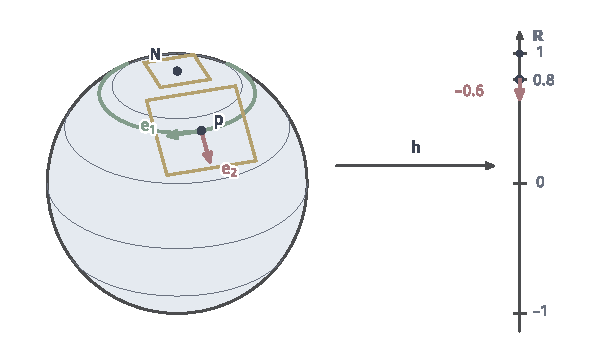
\includegraphics[width=104mm]{figures/04-spaces-measures-and-geometry/04-manifolds/matplotlib/mrel-height-rank/figure.pdf}
  \caption{高度函数$h(\bm y)=y_3$在$S^2$上的秩。在$p=(0,\tfrac35,\tfrac45)$处，绿色的纬线方向$\bm e_1$属于$\ker\mathrm dh_p$，红色的方向$\bm e_2$被送到$\mathbb R$上长度$0.6$的向量（两侧都按真实长度的$0.3$倍画出）。在北极$N$处切平面水平，$\mathrm dh_N=0$，所有方向都被送到零。}
  \label{fig:mrel-height-rank}
\end{BookInlineFigure}

\paragraph{微分的单射、满射与映射的单射、满射}
浸入与淹没都是逐点关于微分的条件，不涉及映射本身是否单射或满射。表~\ref{tab:mrel-injective-comparison}列出了四个例子，说明这两组概念互相独立，判断时要分清问的是方向还是点。

\begin{BookInlineTable}
  \centering
  \begin{tabular}{lll}
    \toprule
    映射 & 映射本身 & 微分\\
    \midrule
    $E:\mathbb R\to\mathbb R^2$ & 非单射（周期$2\pi$） & 处处单射\\
    $\beta(t)=(t^2,t^3)$ & 单射 & 在$t=0$处不单射\\
    $h:S^2\setminus\{N,S\}\to\mathbb R$ & 非满射（像为$(-1,1)$） & 处处满射\\
    $x\mapsto x^3$ & 满射 & 在原点不满射\\
    \bottomrule
  \end{tabular}
  \caption{映射的单射、满射与微分的单射、满射互相独立。}
  \label{tab:mrel-injective-comparison}
\end{BookInlineTable}

\subsection{常秩定理}
\label{sec:mrel-constant-rank}

\paragraph{一点的秩与邻域中的秩}
线性代数告诉我们，任何秩为$r$的矩阵$\bm A$，在定义域和值域各选一组合适的基之后，都成为最简单的形式：存在可逆矩阵$\bm P,\bm Q$，使
\[
\bm P\bm A\bm Q=\begin{bmatrix}\bm I_r&\bm 0\\\bm 0&\bm 0\end{bmatrix}.
\]
选基换成选坐标，我们希望非线性映射也能写成$(x_1,\ldots,x_r,0,\ldots,0)$这样的形式。

类比在这里遇到了线性代数没有的问题：Jacobian矩阵随点变化，矩阵的秩也可能随点变化。一点的秩控制附近秩的下限，却不控制上限。若$\mathrm dF_p$的秩为$r$，Jacobian矩阵有一个非零的$r$阶子式，子式是偏导数的多项式，连续，所以在$p$附近仍非零，附近各点的秩至少为$r$。

秩却可以在$p$附近变大。$f(x)=x^2$在$0$处秩为$0$，在其余点秩为$1$。若它在$0$附近有秩$1$的标准形式$x\mapsto x$，就应当局部单射；若有秩$0$的标准形式，就应当局部为常值。这两者都不成立，因为$f(1/k)=f(-1/k)$，而$f$又不是常值。可见只看一点的秩，得不到局部形式。

二维的例子也一样。令$F(x,y)=(x,xy)$，Jacobian矩阵和行列式分别是
\[
\bm J_F=\begin{bmatrix}1&0\\y&x\end{bmatrix},\qquad \det\bm J_F=x.
\]
在$x=0$处秩为$1$，在$x\neq0$处秩为$2$。球面的高度函数也是如此：在两极秩为$0$，在附近的点秩为$1$，所以两极附近不能用单一的标准形式描述。

有一个重要的例外是满秩。秩不能超过$\min(m,n)$，若$p$处的秩已经达到$\min(m,n)$，附近的秩既不小于它，也不能更大，只能保持不变。所以对浸入和淹没，一点满秩就推出邻域常秩，下面的定理对它们自动适用。

\paragraph{定理与证明}
常秩条件下，映射在适当的坐标中就是线性映射的标准形式。证明的想法是用反函数定理逐步“拉直”：先在源中换坐标，使映射的前$r$个分量变成坐标本身；再由秩的上限，说明其余分量只依赖前$r$个坐标；最后在目标中换坐标，把其余分量减掉。

\begin{theorem}[常秩定理]
\label{thm:mrel-constant-rank}
设$F:M\to N$光滑，$p\in M$，$F$在$p$的某个邻域中各点的秩都等于$r$。则存在以$p$为中心的图$(U,\varphi)$与以$F(p)$为中心的图$(V,\psi)$，$F(U)\subseteq V$，使
\begin{equation}
\psi\circ F\circ\varphi^{-1}(x_1,\ldots,x_r,x_{r+1},\ldots,x_m)=(x_1,\ldots,x_r,0,\ldots,0).
\label{eq:mrel-constant-rank-form}
\end{equation}
\end{theorem}

\begin{proof}
取两侧的图，可设$F$是欧氏开集$W\subseteq\mathbb R^m$到$\mathbb R^n$的光滑映射，$p=\bm 0$，$F(\bm 0)=\bm 0$，并且在$W$上秩恒为$r$。$\bm J_F(\bm 0)$有一个非零的$r$阶子式，重排两侧坐标的次序，可设它位于左上角。

把变量写成$\bm x=(\bm x',\bm x'')$，$\bm x'\in\mathbb R^r$，并把$F$写成$(Q,R)$，其中$Q$取值于$\mathbb R^r$。于是$\partial Q/\partial\bm x'(\bm 0)$可逆。

第一步，在源中换坐标。令$G(\bm x)=(Q(\bm x),\bm x'')$，它在$\bm 0$处的Jacobian矩阵是
\[
\bm J_G(\bm 0)=\begin{bmatrix}\partial Q/\partial\bm x'(\bm 0)&\partial Q/\partial\bm x''(\bm 0)\\\bm 0&\bm I_{m-r}\end{bmatrix},
\]
行列式等于$\det\partial Q/\partial\bm x'(\bm 0)\neq0$。由反函数定理，$G$把$\bm 0$的某个邻域微分同胚地映到$\bm 0$的一个邻域，缩小后可设后者是开方体$C$。

在$C$上有$G\circ G^{-1}=\mathrm{id}$，比较前$r$个分量得$Q(G^{-1}(\bm z))=\bm z'$，所以
\[
F\circ G^{-1}(\bm z)=\bigl(\bm z',\,\widetilde R(\bm z)\bigr),\qquad \widetilde R=R\circ G^{-1}.
\]

第二步，利用秩的上限。$F\circ G^{-1}$的Jacobian矩阵是
\[
\begin{bmatrix}\bm I_r&\bm 0\\\partial\widetilde R/\partial\bm z'&\partial\widetilde R/\partial\bm z''\end{bmatrix}.
\]
$G^{-1}$是微分同胚，所以这个矩阵的秩恒等于$r$。前$r$行已经贡献了秩$r$，若右下块有非零元素，秩就至少为$r+1$，于是
\[
\frac{\partial\widetilde R}{\partial\bm z''}\equiv\bm 0.
\]
$C$是方体，固定$\bm z'$时$\bm z''$在一个凸集中变化，所以$\widetilde R(\bm z)=S(\bm z')$只依赖$\bm z'$。

第三步，在目标中换坐标。令
\[
T(\bm y',\bm y'')=\bigl(\bm y',\ \bm y''-S(\bm y')\bigr),
\]
定义在$\bm y'$属于$C$在前$r$个坐标上的投影的开集上。它光滑，逆为$(\bm y',\bm y''+S(\bm y'))$，也光滑。代入后得到
\[
T\circ F\circ G^{-1}(\bm z)=\bigl(\bm z',\ S(\bm z')-S(\bm z')\bigr)=(\bm z',\bm 0).
\]
取源中的新坐标为$G$，目标中的新坐标为$T$，并缩小邻域使$F(U)\subseteq V$，即得所需形式。
\end{proof}

\paragraph{例子：一步步拉直}
证明中的三步可以在一个具体映射上完整走一遍。令$F:\mathbb R^2\to\mathbb R^2$，
\[
F(x_1,x_2)=(s,s^2),\qquad s=x_1+x_2.
\]
它的Jacobian矩阵第二行是第一行的$2s$倍：
\[
\bm J_F=\begin{bmatrix}1&1\\2s&2s\end{bmatrix},\qquad\operatorname{rank}\bm J_F=1.
\]
所以秩处处等于$1$，常秩定理适用，$r=1$。

这里$Q(x_1,x_2)=x_1+x_2$，$R(x_1,x_2)=(x_1+x_2)^2$，$\partial Q/\partial x_1=1\neq0$。第一步在源中换坐标，
\[
G(x_1,x_2)=(x_1+x_2,\ x_2),\qquad G^{-1}(z_1,z_2)=(z_1-z_2,\ z_2).
\]

把$G^{-1}$代入$F$，第一个分量变成坐标$z_1$，第二个分量自动只依赖$z_1$：
\[
F\circ G^{-1}(z_1,z_2)=(z_1,\ z_1^2).
\]
也就是说第二步中的$S(z_1)=z_1^2$，这里无需额外计算，因为$F$本来就沿直线$x_1+x_2=$常数取常值。第三步在目标中减去$S$，
\[
T(y_1,y_2)=(y_1,\ y_2-y_1^2),\qquad T\circ F\circ G^{-1}(z_1,z_2)=(z_1,0).
\]

图~\ref{fig:mrel-rank-steps}跟踪了点$(1,2)$：$F$把它送到$(3,9)$，$G$把它送到$(3,2)$，$T$把$(3,9)$送到$(3,0)$，而$(z_1,z_2)=(3,2)$在标准形式下正好变成$(3,0)$。图中可以看到映射的结构：源上的等值线是一族平行直线，目标上的像是一条抛物线，换坐标只是把直线摆正、把抛物线压平。

\begin{BookInlineFigure}
  \centering
  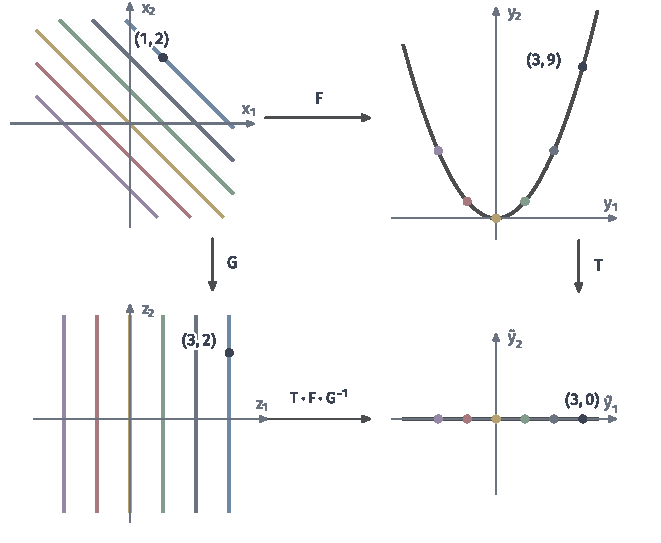
\includegraphics[width=112mm]{figures/04-spaces-measures-and-geometry/04-manifolds/matplotlib/mrel-rank-steps/figure.pdf}
  \caption{常秩定理的三步，$F(x_1,x_2)=(s,s^2)$，$s=x_1+x_2$。左上：源中的等值线$x_1+x_2=c$，$c=-2,\ldots,3$，同一条线上颜色相同。右上：它们被$F$压成抛物线上的一点（同色）。左下：$G$把等值线摆成竖直线。右下：$T$把抛物线压平到坐标轴上。黑点是$(1,2)$的轨迹。}
  \label{fig:mrel-rank-steps}
\end{BookInlineFigure}

\paragraph{浸入与淹没的局部形式}
由上面的满秩讨论，浸入在每点附近秩恒为$m$，淹没恒为$n$，常秩定理直接给出它们的局部形式：
\begin{align}
\text{浸入：}\quad&(x_1,\ldots,x_m)\mapsto(x_1,\ldots,x_m,0,\ldots,0),\label{eq:mrel-immersion-form}\\
\text{淹没：}\quad&(x_1,\ldots,x_n,\ldots,x_m)\mapsto(x_1,\ldots,x_n).\label{eq:mrel-submersion-form}
\end{align}

图~\ref{fig:mrel-normal-forms}画出这两种形式和一般常秩映射。式~\eqref{eq:mrel-immersion-form}说，浸入局部上把$\mathbb R^m$放进$\mathbb R^n$作为前$m$个坐标的子空间，所以局部单射，像的一小块是一片平的$m$维片。式~\eqref{eq:mrel-submersion-form}说，淹没局部上沿后$m-n$个坐标投影，每点的原像局部是一片$m-n$维的片。

\begin{BookInlineFigure}
  \centering
  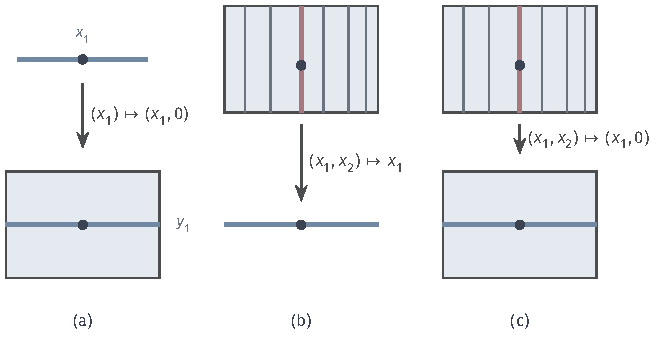
\includegraphics[width=111.767mm]{figures/04-spaces-measures-and-geometry/04-manifolds/tikz/mrel-normal-forms/figure.pdf}
  \caption{常秩映射的局部标准形式。(a)浸入：区间平放进平面，成为一条坐标线。(b)淹没：矩形沿竖直方向投影到区间上，红色竖线是一点的原像。(c)一般的常秩映射（$m=n=2$，$r=1$）：竖线整条压成一点，像是一条横线，定义域和值域都没有被占满。}
  \label{fig:mrel-normal-forms}
\end{BookInlineFigure}

前面的例子都可以写成这样的形式。对$E$，在圆周上用$\mathbb R^2$的极坐标图$(\theta,r-1)$，$E$的坐标表示恰好是$t\mapsto(t,0)$，这就是式~\eqref{eq:mrel-immersion-form}。对高度函数$h$，在$p$附近用坐标$(h,\lambda)$，其中$\lambda$是经度，$h$的坐标表示就是投影$(h,\lambda)\mapsto h$，这就是式~\eqref{eq:mrel-submersion-form}。

表~\ref{tab:mrel-immersion-submersion}把两种映射并排比较。下一节正是用这两种局部形式构造子流形：浸入给出“像”的局部坐标，淹没给出“水平集”的局部坐标。

\begin{BookInlineTable}
  \centering
  \begin{tabular}{lll}
    \toprule
    & 浸入 & 淹没\\
    \midrule
    微分 & 处处单射 & 处处满射\\
    秩 & 恒为$m$ & 恒为$n$\\
    维数 & $m\leq n$ & $m\geq n$\\
    Jacobian矩阵 & 列满秩 & 行满秩\\
    局部形式 & 加上若干零坐标 & 丢掉若干坐标\\
    局部几何 & 像是平的$m$维片 & 原像是平的$(m-n)$维片\\
    \bottomrule
  \end{tabular}
  \caption{浸入与淹没的比较。}
  \label{tab:mrel-immersion-submersion}
\end{BookInlineTable}

\section{嵌入子流形}
\label{sec:mrel-embedded-submanifolds}

浸入在每点附近都像把一块平的片放进目标空间，可这些局部的片拼起来，未必是目标中一个像样的子空间：像可能自己穿过自己，也可能从远处绕回来贴近自身。本节先在浸入之上加入整体的拓扑条件，得到嵌入；再在目标的坐标中描述嵌入子流形的局部样子；最后研究由约束方程定义的集合何时是这样的子流形。

\subsection{嵌入}
\label{sec:mrel-embedding}

\paragraph{“8”字形曲线}
考虑$\alpha:(-\pi,\pi)\to\mathbb R^2$，$\alpha(t)=(\sin2t,\sin t)$。速度$(2\cos2t,\cos t)$处处非零：若$\cos t=0$，则$t=\pm\pi/2$，此时$\cos2t=-1$。所以$\alpha$是浸入。它还是单射：若$\sin t=\sin s$且$t\neq s$，则$s=\pi-t$或$s=-\pi-t$，于是$\sin2s=-\sin2t$，要使第一个分量也相等只能$\sin2t=0$，即$t\in\{0,\pm\pi/2\}$。$t=0$时$s=\pm\pi$不在区间内，$t=\pm\pi/2$时$s=t$，都与假设矛盾。特别地，$t=0$是唯一映到原点的参数。

$\alpha$的像是一个“8”字：$t$从$0$增大到$\pi$时画出一个圈，$t\to\pi$时又回到原点附近；$t$从$0$减小到$-\pi$时画出另一个圈。取$t_k\to\pi$，则$\alpha(t_k)\to(0,0)=\alpha(0)$，但$t_k$不趋于$0$。从像的角度看，点列收敛到原点；从参数的角度看，对应的参数却跑到了区间的另一端。所以$\alpha$作为从$(-\pi,\pi)$到其像的双射，逆映射不连续。

\paragraph{定义}
“8”字形曲线的问题不在局部方向，而在像所继承的拓扑与源流形的拓扑不一致。像$F(M)$作为$N$的子集，有从$N$继承的子空间拓扑：$F(M)$中的开集是$N$中开集与$F(M)$的交。要求$F$在这一拓扑下是同胚，就排除了上述情形。

\begin{definition}[嵌入]
\label{def:mrel-embedding}
光滑映射$F:M\to N$称为\term{嵌入}（embedding），若$F$是浸入，并且$F:M\to F(M)$是同胚，其中$F(M)$带有从$N$继承的子空间拓扑。
\end{definition}

于是有三个层层加强的条件：浸入只要求微分单射；单射浸入还要求映射本身单射；嵌入进一步要求到像的同胚。$E:\mathbb R\to\mathbb R^2$，$t\mapsto(\cos t,\sin t)$是浸入但不是单射，像自己反复重叠；$\alpha$是单射浸入但不是嵌入；把$E$限制到$(0,2\pi)$上，得到单射浸入，它的逆就是角度图$\theta_2$，连续，所以是嵌入。

\paragraph{紧流形的单射浸入}
源流形紧时，后两个条件之间的差距消失。

\begin{theorem}[紧流形上的单射浸入]
\label{thm:mrel-compact-injective-immersion}
若$M$紧，$F:M\to N$是单射浸入，则$F$是嵌入。
\end{theorem}

\begin{proof}
只需证明$F:M\to F(M)$的逆连续，即$F$把$M$的闭集映为$F(M)$的闭集。设$K\subseteq M$是闭集，紧空间的闭子集是紧集，所以$K$紧；连续映射把紧集映为紧集，$F(K)$紧；$N$是Hausdorff空间，其紧子集是闭集，所以$F(K)$在$N$中闭，从而在$F(M)$中闭。
\end{proof}

$\alpha$的源区间$(-\pi,\pi)$不紧，参数可以逃向端点而像却回到原点，定理正是排除了这种逃逸。

\subsection{子流形的局部表示}
\label{sec:mrel-submanifold-local}

\paragraph{切片坐标}
嵌入的像在目标中应当局部像一块平的片。用目标的坐标表达：在合适的图中，像恰好是一部分坐标为零的那片点。

\begin{definition}[嵌入子流形]
\label{def:mrel-embedded-submanifold}
设$M$是$n$维光滑流形，$S\subseteq M$，$0\leq k\leq n$。若对每个$p\in S$，都有$M$的图$(U,\varphi)$，$p\in U$，使
\begin{equation}
\varphi(U\cap S)=\{\bm x\in\varphi(U):x_{k+1}=\cdots=x_n=0\},
\label{eq:mrel-slice-chart}
\end{equation}
则称$S$为$M$的$k$维\term{嵌入子流形}（embedded submanifold）。这样的图称为$S$的\term{切片坐标}（slice chart）。$n-k$称为$S$的\term{余维数}（codimension）。
\end{definition}

切片坐标中的前$k$个坐标在$S$上自由变化，是$S$的内部坐标；后$n-k$个坐标描述离开$S$的方向，在$S$上为零。这一描述与嵌入是同一件事的两面。

\begin{theorem}[嵌入与嵌入子流形]
\label{thm:mrel-embedding-submanifold}
\begin{enumerate}
\item 设$S$是$M$的$k$维嵌入子流形，带子空间拓扑。把切片坐标限制到$U\cap S$并只保留前$k$个坐标，得到$S$的光滑图册，$S$成为$k$维光滑流形，包含映射$\iota:S\to M$是嵌入。
\item 若$F:P\to M$是嵌入，则$F(P)$是$M$的嵌入子流形，维数等于$\dim P$，并且$F:P\to F(P)$是微分同胚。
\end{enumerate}
\end{theorem}

\begin{proof}
第一条。限制后的映射是$U\cap S$到$\mathbb R^k$开集的同胚，因为$\varphi$是同胚，而式\eqref{eq:mrel-slice-chart}说明$U\cap S$恰好对应坐标平面$\mathbb R^k\times\{\bm 0\}$与$\varphi(U)$的交。两张这样的图之间的坐标变换，是$M$的坐标变换限制到$\mathbb R^k\times\{\bm 0\}$上再取前$k$个分量，仍光滑。$S$作为$M$的子空间是Hausdorff且第二可数的。在这些图中，$\iota$的坐标表示是$\bm x'\mapsto(\bm x',\bm 0)$，是浸入；$S$本来就带子空间拓扑，$\iota$到像的同胚是自然的。

第二条。设$p\in P$，$k=\dim P$。$F$是浸入，由常秩定理，有以$p$为中心的图$(U,\varphi)$与以$F(p)$为中心的图$(V,\psi)$，使$\psi\circ F\circ\varphi^{-1}(\bm x')=(\bm x',\bm 0)$。这只说明$F(U)$是一片，还须排除$F(P)$的其他部分从远处进入$V$。这就要用到同胚条件：$F(U)$在$F(P)$中开，所以存在$M$中的开集$W$，使$F(U)=W\cap F(P)$。

令$V'=V\cap W\cap\psi^{-1}\bigl(\varphi(U)\times\mathbb R^{n-k}\bigr)$。若$q\in V'\cap F(P)$，则$q\in W\cap F(P)=F(U)$，所以$\psi(q)=(\bm x',\bm 0)$，$\bm x'\in\varphi(U)$。反过来，若$q\in V'$且$\psi(q)=(\bm x',\bm 0)$，则$\bm x'\in\varphi(U)$，$q=\psi^{-1}(\bm x',\bm 0)=F(\varphi^{-1}(\bm x'))\in F(P)$。所以$\psi$限制到$V'$上是$F(P)$的切片坐标。最后，在$P$的图$\varphi$与$F(P)$的限制图下，$F$的坐标表示是恒等映射，故$F$是到像的微分同胚。
\end{proof}

\paragraph{子流形的切空间}
包含映射$\iota$是浸入，$\mathrm d\iota_p$把$T_pS$单射地送入$T_pM$。今后把$T_pS$与它的像$\mathrm d\iota_p(T_pS)$等同，看作$T_pM$的$k$维子空间。在切片坐标中，$\iota$的坐标表示是$\bm x'\mapsto(\bm x',\bm 0)$，所以
\[
T_pS=\operatorname{span}\bigl\{\partial_1|_p,\ldots,\partial_k|_p\bigr\}\subseteq T_pM .
\]
沿后$n-k$条坐标线运动会离开$S$，相应的方向不在$T_pS$中。当$M=\mathbb R^n$时，$T_pM$就是$\mathbb R^n$，$T_pS$成为$\mathbb R^n$的一个线性子空间，这就是嵌入在欧氏空间中的曲线与曲面的切向量的通常含义。

\paragraph{例子：圆周、球面、图像与乘积}
圆周$S^1\subseteq\mathbb R^2$。在去掉负半轴$\{(y_1,0):y_1\leq0\}$的平面上用极坐标$(\theta,r)$，令$\varphi(\bm y)=(\theta,r-1)$。在这张图中，$S^1$恰好对应第二个坐标为零，所以它是切片坐标；另一张图用去掉正半轴的极坐标。于是$S^1$是$\mathbb R^2$的一维嵌入子流形，余维数为$1$。三种坐标在这里分得很清楚：$\theta$是圆周的内部坐标，$(y_1,y_2)$是环境坐标，$r-1$是只在环境中有意义的离开圆周的坐标。球面$S^2\subseteq\mathbb R^3$用球坐标$(\theta,\phi,r-1)$类似处理。

光滑函数$f:W\to\mathbb R^{n-k}$（$W\subseteq\mathbb R^k$开）的图像$\Gamma_f=\{(\bm x,f(\bm x)):\bm x\in W\}$是$W\times\mathbb R^{n-k}$的嵌入子流形：$\varphi(\bm x,\bm y)=(\bm x,\bm y-f(\bm x))$是微分同胚，逆为$(\bm x,\bm z)\mapsto(\bm x,\bm z+f(\bm x))$，它把$\Gamma_f$送到$\{\bm z=\bm0\}$。这个例子说明，局部上“是图像”与“有切片坐标”是一回事，下一小节的隐函数表示正是把子流形局部写成图像。

乘积也保持子流形关系。若$S_1\subseteq M_1$与$S_2\subseteq M_2$分别是嵌入子流形，两张切片坐标的乘积是$S_1\times S_2$在$M_1\times M_2$中的切片坐标，只需把坐标重新排序，使取零的坐标放在最后。例如环面$S^1\times S^1$是$\mathbb R^2\times\mathbb R^2=\mathbb R^4$的二维嵌入子流形，余维数为$2$。

\paragraph{不是子流形的子集}
子流形的定义对每个点都要求切片坐标，任意子集未必满足。十字形$X=\{(y_1,y_2):y_1y_2=0\}$在原点以外是两条坐标轴，局部是直线；但在原点处，它不是一维子流形。若是，原点在$X$中有一个连通邻域同胚于开区间，去掉原点后恰有两个连通分支；可原点在$X$中的任何足够小的连通邻域，去掉原点后都有四个分支，即四条半轴的片段。“8”字形曲线的像在原点处也是同样的十字形交叉，所以$\alpha$的像不是嵌入子流形，与$\alpha$不是嵌入相符。

还有更隐蔽的情形。尖点曲线$\{y_2^2=y_1^3\}$作为拓扑空间同胚于实轴，没有十字交叉，但可以证明它在原点处没有切片坐标，因而不是$\mathbb R^2$的光滑嵌入子流形，这里不给出证明。上一节的参数化$\beta(t)=(t^2,t^3)$恰好在原点速度为零，与此相呼应。可见判断是否为子流形，既要看拓扑，也要看光滑结构。

\subsection{正则水平集}
\label{sec:mrel-regular-level-sets}

很多子流形由约束方程给出：球面是$\lVert\bm y\rVert_2^2=1$的解集，正交矩阵是$\bm A^\top\bm A=\bm I$的解集。问题是：约束方程的解集何时是子流形，维数是多少，切空间是什么？

\paragraph{正则值}
设$\Phi:M\to N$光滑，$c\in N$。水平集$\Phi^{-1}(c)$由所有满足约束$\Phi(p)=c$的点组成。若每个约束都提供一个独立的方向限制，就应当把$m$个自由度减去$n$个。“独立”的准确含义是微分满秩。

\begin{definition}[正则值与正则水平集]
\label{def:mrel-regular-value}
设$\Phi:M\to N$光滑。若$\mathrm d\Phi_p$是满射，称$p$为$\Phi$的正则点，否则称为临界点。若$\Phi^{-1}(c)$中的每一点都是正则点，称$c$为$\Phi$的\term{正则值}（regular value），$\Phi^{-1}(c)$称为\term{正则水平集}（regular level set）。
\end{definition}

按定义，不在像中的点也是正则值，这时水平集为空，下面的定理对空集自然成立。

\begin{theorem}[正则水平集定理]
\label{thm:mrel-regular-level-set}
设$\Phi:M\to N$光滑，$c$是$\Phi$的正则值。则$S=\Phi^{-1}(c)$是$M$的$m-n$维嵌入子流形，并且对每个$p\in S$，
\[
T_pS=\ker\mathrm d\Phi_p .
\]
\end{theorem}

\begin{proof}
正则点组成的集合$M_0$是开集，因为满秩在附近保持。$S\subseteq M_0$，$\Phi$在$M_0$上是淹没，由常秩定理，每个$p\in S$附近有图$\varphi$与以$c$为中心的图$\psi$，使$\psi\circ\Phi\circ\varphi^{-1}(x_1,\ldots,x_m)=(x_1,\ldots,x_n)$。于是$S$在这张图中恰好是$x_1=\cdots=x_n=0$的点。把坐标重新排序，让这$n$个坐标排在最后，就得到$m-n$维的切片坐标。

$\Phi$在$S$上取常值$c$，所以$\Phi\circ\iota$是常值映射，微分为零，即$\mathrm d\Phi_p\circ\mathrm d\iota_p=0$，$T_pS\subseteq\ker\mathrm d\Phi_p$。$\mathrm d\Phi_p$满射，由秩--零度关系，核的维数是$m-n$，与$T_pS$相同，所以二者相等。
\end{proof}

定理与隐函数定理是同一件事的两种说法。在欧氏情形，$\Phi:\mathbb R^m\to\mathbb R^n$在$p$处的Jacobian矩阵行满秩，可以选出$n$列组成可逆方阵；隐函数定理把对应的$n$个变量解成其余$m-n$个变量的光滑函数，水平集在$p$附近就是这个函数的图像，再由上一小节的图像例子得到切片坐标。满秩条件排除了局部奇点：在不满秩的点，约束之间可能互相重复，也可能在该点退化，解集在那里可以出现交叉或孤立点。

\paragraph{球面}
令$\Phi:\mathbb R^3\to\mathbb R$，$\Phi(\bm y)=\lVert\bm y\rVert_2^2$。$\mathrm d\Phi_{\bm y}(\bm v)=2\bm y^\top\bm v$，当$\bm y\neq\bm 0$时它是到$\mathbb R$的满射。$\Phi^{-1}(1)=S^2$不含原点，所以$1$是正则值，$S^2$是二维嵌入子流形，并且
\[
T_{\bm p}S^2=\{\bm v\in\mathbb R^3:\bm p^\top\bm v=0\},
\]
即与$\bm p$正交的平面。这与第~\ref{chap:manifold-basics}章用球极投影算出的切向量$(0.2,0,0)$与$\bm p=(0,\tfrac35,\tfrac45)$正交一致。同样，椭球面是$\sum_iy_i^2/a_i^2=1$的正则水平集；线性映射$\bm y\mapsto(y_1/a_1,y_2/a_2,y_3/a_3)$把它一一映到球面，在两侧的子流形结构下是微分同胚，这就是本章开头说椭球面与球面“本质上相同”的含义。

\paragraph{正则性只是充分条件}
不满足正则性时，水平集可能不是子流形。$\Phi(y_1,y_2)=y_1^2-y_2^2$在原点处微分为零，$\Phi^{-1}(0)$是两条直线$y_2=\pm y_1$的并，在原点处交叉，与上一小节的十字形一样不是子流形。$\Phi(\bm y)=\lVert\bm y\rVert_2^2$的零水平集只有原点，是零维子流形，却不是定理预测的二维；那里原点是临界点，定理本来就不适用。

水平集也可能在正则性失败时仍是子流形。$\Phi(\bm y)=(\lVert\bm y\rVert_2^2-1)^2$的零水平集仍是单位圆，但在圆上$\mathrm d\Phi=4(\lVert\bm y\rVert_2^2-1)\bm y^\top=\bm 0$，没有一个点是正则点。这说明正则值是水平集为子流形的充分条件，不是必要条件；同一个集合换一个约束函数，正则性可能成立，也可能不成立。

\paragraph{正交矩阵与重复方程}
全体$n$阶正交矩阵组成的集合$\mathrm O(n)=\{\bm A\in\mathbb R^{n\times n}:\bm A^\top\bm A=\bm I\}$称为\term{正交群}（orthogonal group）。它由$n^2$个方程定义，但这些方程有重复：$\bm A^\top\bm A$总是对称矩阵，第$(i,j)$个方程与第$(j,i)$个方程相同。若把约束映射看成取值于$\mathbb R^{n\times n}$，它的微分只能取到对称矩阵，永远不是满射，单位矩阵不是正则值，定理用不上。

正确的做法是让约束映射取值于对称矩阵组成的空间$\operatorname{Sym}(n)$，它是$n(n+1)/2$维线性空间。令$\Phi:\mathbb R^{n\times n}\to\operatorname{Sym}(n)$，$\Phi(\bm A)=\bm A^\top\bm A$。对方向$\bm H$求导，
\[
\mathrm d\Phi_{\bm A}(\bm H)=\bm H^\top\bm A+\bm A^\top\bm H .
\]
在$\bm A\in\mathrm O(n)$处，任给对称矩阵$\bm C$，取$\bm H=\tfrac12\bm A\bm C$，利用$\bm A^\top\bm A=\bm I$与$\bm C^\top=\bm C$，得
\[
\mathrm d\Phi_{\bm A}\bigl(\tfrac12\bm A\bm C\bigr)=\tfrac12\bm C^\top\bm A^\top\bm A+\tfrac12\bm A^\top\bm A\bm C=\bm C .
\]
所以$\mathrm d\Phi_{\bm A}$是满射，$\bm I$是正则值。

由定理~\ref{thm:mrel-regular-level-set}，$\mathrm O(n)$是$\mathbb R^{n\times n}$的嵌入子流形，维数为$n^2-n(n+1)/2=n(n-1)/2$。在单位矩阵处，$T_{\bm I}\mathrm O(n)=\ker\mathrm d\Phi_{\bm I}=\{\bm H:\bm H^\top+\bm H=\bm 0\}$，即全体反对称矩阵，维数恰为$n(n-1)/2$，与上面一致。$n=2$时维数为$1$，对应平面旋转的一个转角参数；$n=3$时维数为$3$，对应三维旋转的三个自由度。$\mathrm O(n)$既是流形又是群，这种结构在第~\ref{chap:lie-groups}章研究。

\paragraph{带边界的情形}
本章的结论都针对无边界流形。约束若是不等式，例如闭球$\{\bm y:\lVert\bm y\rVert_2^2\leq1\}$，所得集合是带边界流形，边界恰是正则水平集$\{\lVert\bm y\rVert_2^2=1\}$。一般地，若$c$是光滑实值函数$\Phi:M\to\mathbb R$的正则值，下水平集$\{\Phi\leq c\}$是与$M$同维的带边界流形，边界为$\Phi^{-1}(c)$；证明要在边界点处单独构造半空间坐标，这里不给出。约束集合本身带边界，或映射的定义域带边界时，上述定理都需要另核条件。

\section{本章小结}
\label{sec:mrel-summary}

本章开头问了两个问题：两个流形何时在光滑意义下相同，一个对象何时是另一个流形中的光滑子集。第一个问题由微分同胚回答。它是光滑且逆光滑的双射，比同胚多保留了光滑结构，比集合双射多保留了拓扑；$x\mapsto x^3$是光滑的同胚，却不是微分同胚。

微分同胚在每点的微分都是线性同构，所以维数相同。反过来，反函数定理只说明微分在一点可逆时映射在该点附近是微分同胚。$E(t)=(\cos t,\sin t)$与圆周的倍角映射都是局部微分同胚，却不是单射，整体的双射性必须另外核对。微分同胚也不保持长度，$(0,1)$与$\mathbb R$微分同胚。

映射的局部结构由微分的秩决定。浸入的微分处处单射，淹没的微分处处满射，它们分别要求源的维数不超过或不小于目标的维数，并且与映射本身是否单射、满射无关。一点的秩只给出附近秩的下限，$x\mapsto x^2$在原点秩为零、附近秩为一，没有局部标准形式。

在秩保持不变的邻域中，常秩定理用反函数定理把映射化为“前$r$个坐标不变、其余坐标为零”的标准形式。满秩是开条件，所以浸入与淹没自动满足常秩条件，分别局部像坐标子空间的包含与坐标投影。

第二个问题需要整体条件。“8”字形曲线是单射浸入，参数却可以逃向端点而像回到原点，它到像的逆不连续；环面上的无理斜率直线则处处如此。嵌入在浸入之上要求到像的同胚，紧流形上的单射浸入自动是嵌入。

嵌入的像正是嵌入子流形，即每点附近有切片坐标、子流形对应一部分坐标为零的集合；切空间是前几个坐标基向量张成的子空间。圆周、球面、函数图像与乘积都有切片坐标，十字形和“8”字的交叉点则没有，尖点虽然拓扑上是直线，也没有切片坐标。

约束方程提供了构造子流形的一般办法。若$c$是$\Phi:M\to N$的正则值，水平集$\Phi^{-1}(c)$是$m-n$维嵌入子流形，切空间是$\ker\mathrm d\Phi_p$。球面与椭球面由此得到；正交群$\mathrm O(n)$也由此得到，但约束映射要取值于对称矩阵空间，以免把重复的方程计入满秩要求，所得维数为$n(n-1)/2$，单位元处的切空间是反对称矩阵。正则值只是充分条件，$(\lVert\bm y\rVert_2^2-1)^2$的零水平集是圆，却没有正则点。

本章始终在无边界情形下讨论，带边界时反函数定理与正则水平集定理都要另核条件。所有结论都只涉及光滑结构，不涉及长度和角度。在第~\ref{chap:riemannian-geometry}章给切空间配上内积之后，才能问一个微分同胚是否保持长度，即两个黎曼流形是否等距。

